
\chapter{Milestone 4}
\section{Lenard Jones Derivation}
% Derivation of the analytical expression fot the forces of the lenard-jones Potential
% pyhton code i guess lol
    \begin{tcolorbox}[breakable, size=fbox, boxrule=1pt, pad at break*=1mm,colback=cellbackground, colframe=cellborder]
	\prompt{In}{incolor}{4}{\boxspacing}
	\begin{Verbatim}[commandchars=\\\{\}]
		\PY{k+kn}{import} \PY{n+nn}{sympy} \PY{k}{as} \PY{n+nn}{sp}
		\PY{k+kn}{import} \PY{n+nn}{warnings}
		\PY{n}{warnings}\PY{o}{.}\PY{n}{filterwarnings}\PY{p}{(}\PY{l+s+s1}{\PYZsq{}}\PY{l+s+s1}{ignore}\PY{l+s+s1}{\PYZsq{}}\PY{p}{)}
		\PY{n}{sp}\PY{o}{.}\PY{n}{init\PYZus{}printing}\PY{p}{(}\PY{p}{)}
		\PY{n}{eps} \PY{o}{=} \PY{n}{sp}\PY{o}{.}\PY{n}{Symbol}\PY{p}{(}\PY{l+s+s2}{\PYZdq{}}\PY{l+s+s2}{e}\PY{l+s+s2}{\PYZdq{}}\PY{p}{)}
		\PY{n}{sig} \PY{o}{=} \PY{n}{sp}\PY{o}{.}\PY{n}{Symbol}\PY{p}{(}\PY{l+s+s2}{\PYZdq{}}\PY{l+s+s2}{s}\PY{l+s+s2}{\PYZdq{}}\PY{p}{)}
		\PY{n}{rad} \PY{o}{=} \PY{n}{sp}\PY{o}{.}\PY{n}{Symbol}\PY{p}{(}\PY{l+s+s2}{\PYZdq{}}\PY{l+s+s2}{r}\PY{l+s+s2}{\PYZdq{}}\PY{p}{)}
		\PY{n}{energyRad} \PY{o}{=} \PY{l+m+mi}{4} \PY{o}{*} \PY{n}{eps} \PY{o}{*} \PY{p}{(}\PY{p}{(}\PY{n}{sig}\PY{o}{/}\PY{n}{rad}\PY{p}{)}\PY{o}{*}\PY{o}{*}\PY{l+m+mi}{12} \PY{o}{\PYZhy{}} \PY{p}{(}\PY{n}{sig}\PY{o}{/}\PY{n}{rad}\PY{p}{)}\PY{o}{*}\PY{o}{*}\PY{l+m+mi}{6}\PY{p}{)}
		\PY{n}{energyRad}\PY{o}{.}\PY{n}{diff}\PY{p}{(}\PY{n}{rad}\PY{p}{)}
	\end{Verbatim}
\end{tcolorbox}


\prompt{Out}{outcolor}{4}{}

$\displaystyle 4 e \left(\frac{6 s^{6}}{r^{7}} - \frac{12 s^{12}}{r^{13}}\right)$




\section{Different Time Steps}
%plots for different timesteps
\begin{figure}[!h]
	\begin{center}
		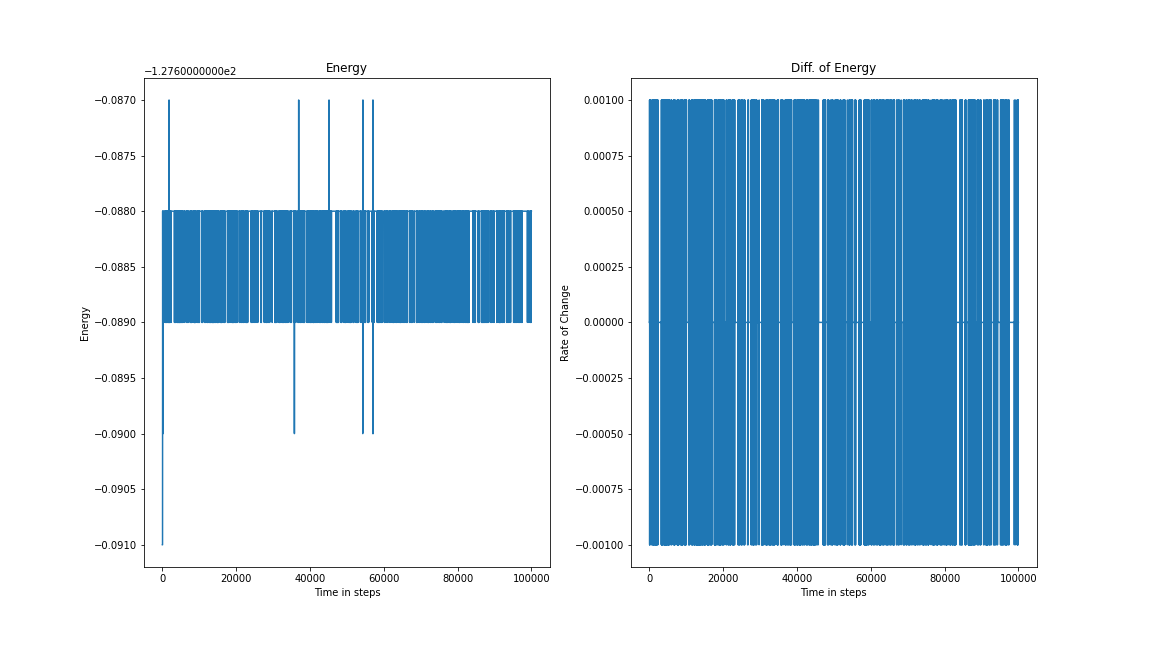
\includegraphics[scale=0.35]{Figure/plot_001.png}
	\end{center}
	\caption[Simulation]{Simulation with a time step of 0.001}
	\label{Plot001}
\end{figure}
\begin{figure}[!h]
	\begin{center}
		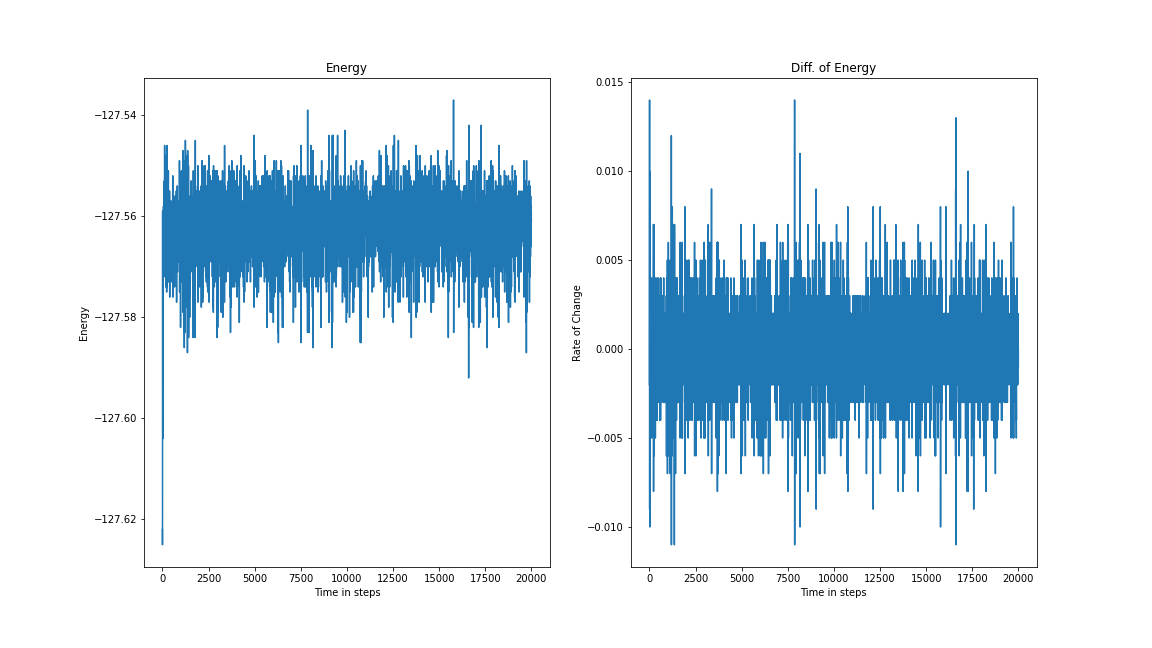
\includegraphics[scale= 0.35]{Figure/plot_005.png}
	\end{center}
	\caption[Simulation]{Simulation with a time step of 0.005}
	\label{Plot005}
\end{figure}
\begin{figure}[!h]
	\begin{center}
		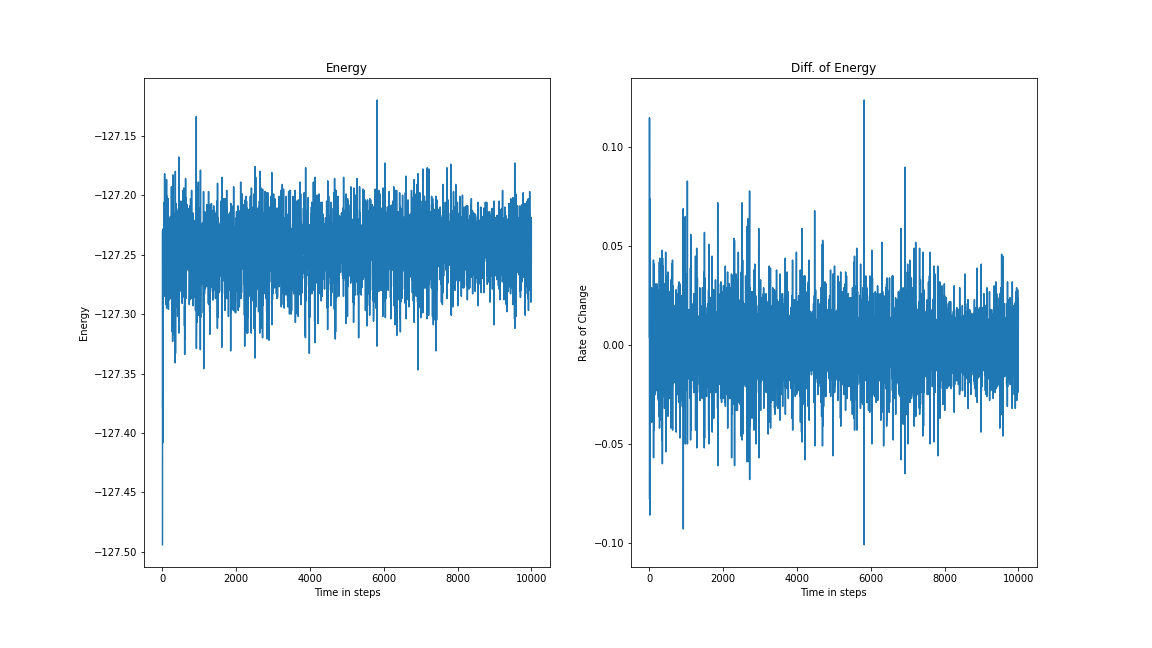
\includegraphics[scale= 0.35]{Figure/plot_01.png}
	\end{center}
	\caption[Simulation]{Simulation with a time step of 0.01}
	\label{Plot01}
\end{figure}
\begin{figure}[!h]
	\begin{center}
		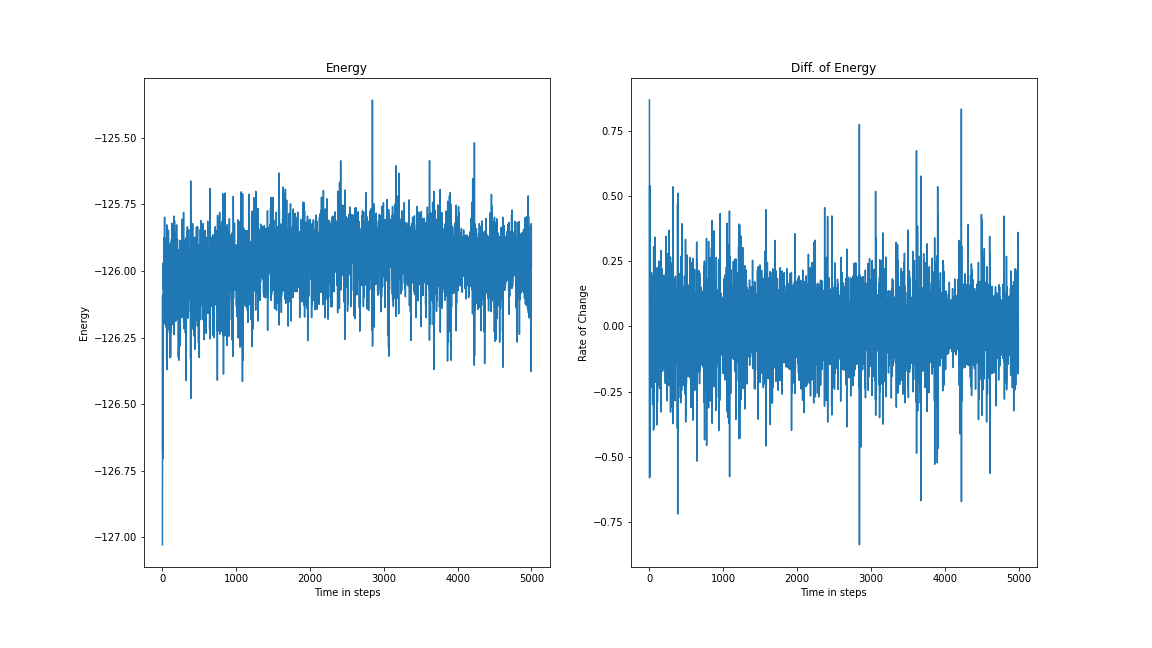
\includegraphics[scale= 0.35]{Figure/plot_02.png}
	\end{center}
	\caption[Simulation]{Simulation with a time step of 0.02 }
	\label{Plot02}
\end{figure}
\begin{figure}[!h]
	\begin{center}
		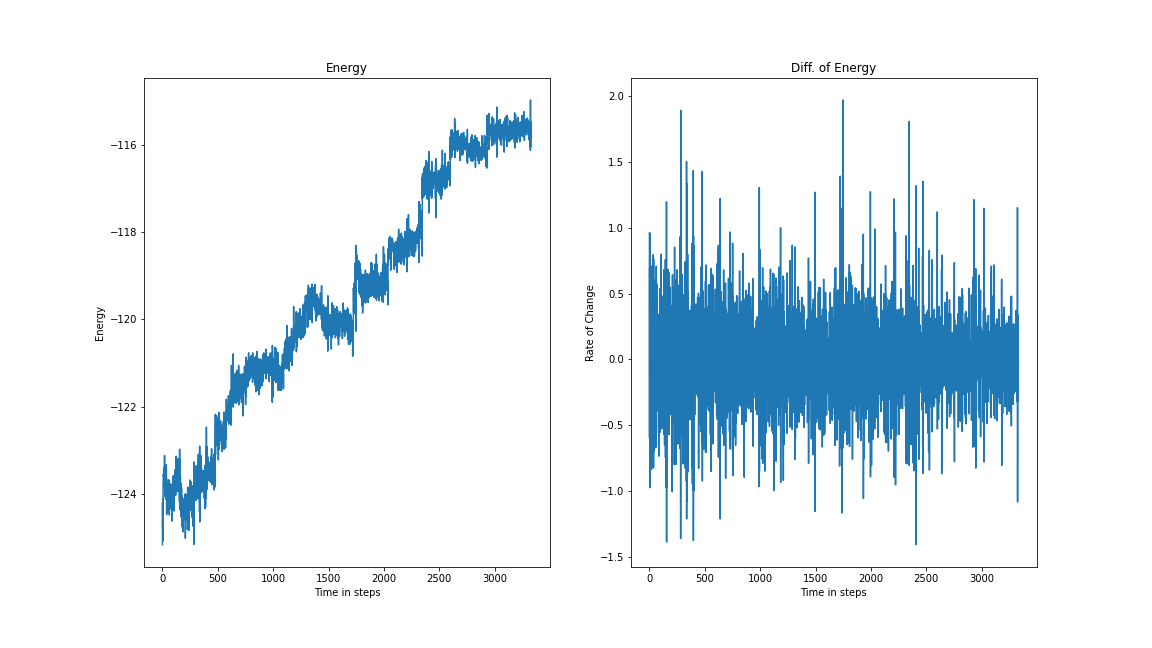
\includegraphics[scale= 0.35]{Figure/plot_03.png}
	\end{center}
	\caption[Simulation]{Simulation with a time step of 0.03 }
	\label{Plot03}
\end{figure}
\begin{figure}[!h]
	\begin{center}
		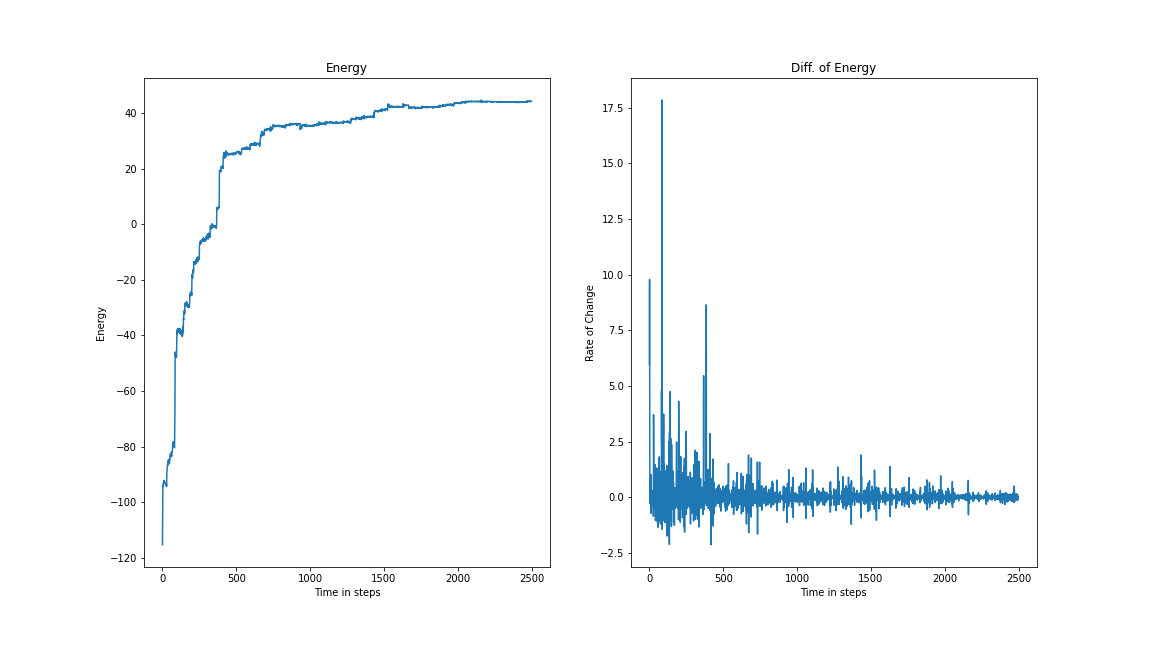
\includegraphics[scale= 0.35]{Figure/plot_04.png}
	\end{center}
	\caption[Simulation]{Simulation with a time step of 0.04 }
	\label{Plot04}
\end{figure}
%Snapshots of the simulation (5)
\section{Simulation Snapshots}
\begin{figure}[!h]
	\begin{center}
		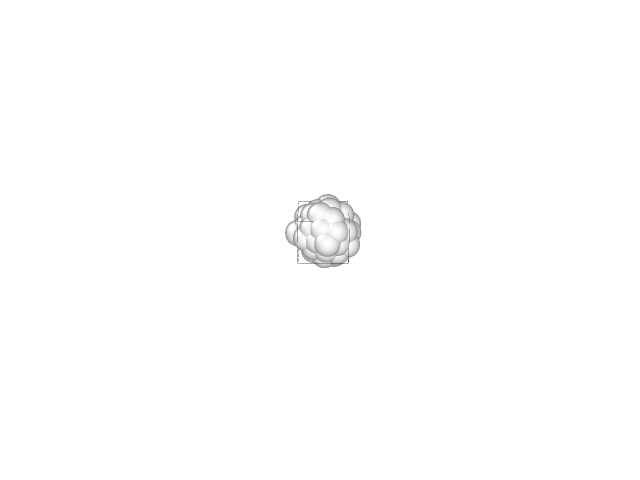
\includegraphics[scale= 1]{Figure/1Image.png}
	\end{center}
	\caption[Simulation]{Simulation }
	\label{Simulation1}
\end{figure}
\begin{figure}[!h]
	\begin{center}
		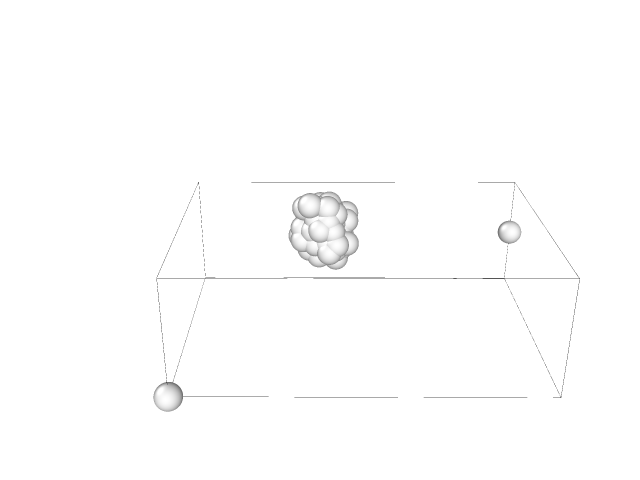
\includegraphics[scale=1]{Figure/2Image.png}
	\end{center}
	\caption[Simulation]{Simulation }
	\label{Simulation2}
\end{figure}
\begin{figure}[!h]
	\begin{center}
		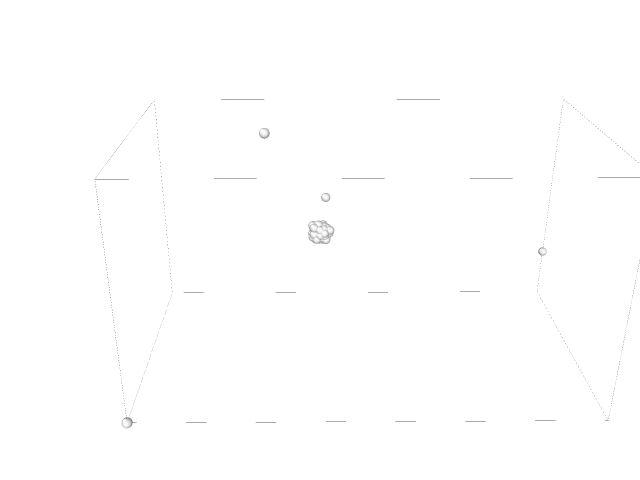
\includegraphics[scale= 1]{Figure/3Image.png}
	\end{center}
	\caption[Simulation]{Simulation }
	\label{Simulation3}
\end{figure}
\begin{figure}[!h]
	\begin{center}
		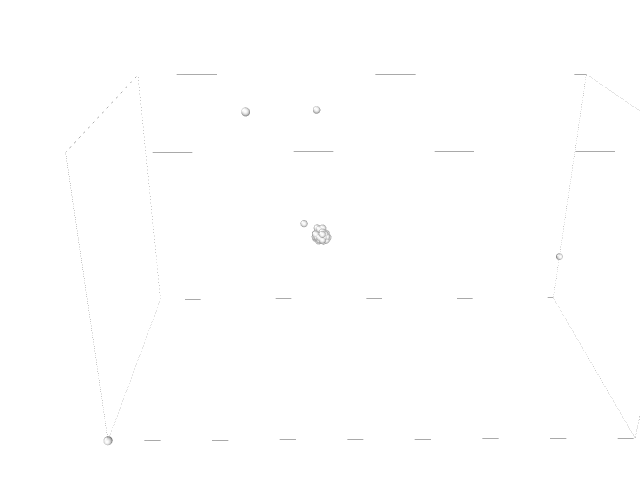
\includegraphics[scale= 1]{Figure/4Image.png}
	\end{center}
	\caption[Simulation]{Simulation }
	\label{Simulation4}
\end{figure}
\begin{figure}[!h]
	\begin{center}
		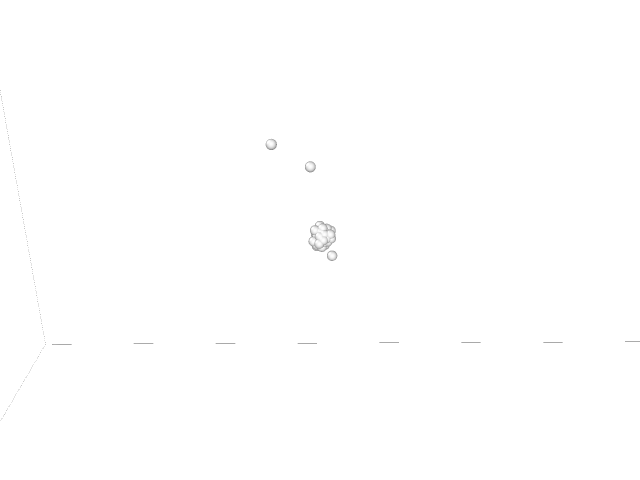
\includegraphics[scale= 1]{Figure/5Image.png}
	\end{center}
	\caption[Simulation]{Simulation }
	\label{Simulation5}
\end{figure}